% \section{Problem Definition}
\section{Dynamic Multi-Domain Problem}
We clarify the \textit{DMPC} problem as follows. Given a set $\mathcal{G}$ of $n$ relatively independent label taxonomies at initial time $t_0$
$$
\{G_1, G_2, G_3, ..., G_n\},
$$
each of which correlates with a domain-specific product categorization task. The taxonomy of product categories $G_i$ is tree-structured with depth $d_i$, and it contains $m_i$ category leaf nodes:
$$
\{y_i^{(1)}, y_i^{(2)}, y_i^{(3)}, ..., y_i^{(m_i)}\} \subseteq G_i.
$$
% As time $t_{>0}$ goes, the category node $y_i^{(a)}$ might be \textbf{divided} into two categories $y_i^{(a1)}$ and $y_i^{(a2)}$ or be  \textbf{integrated} with another category $y_i^{(b)}$ to form $y_i^{(ab)}$. The \textbf{new} category node $y_i^{(m+1)}$ with corresponding products can also appear and the extreme scenario is that an emerging taxonomy $G_{n+1}$ sprouts along with the new business development from another domain.
Part of the nodes is enrolling in a dynamic trending. As time goes $t_{>0}$, the category node $y_i^{(a)}$ of a certain product might be \textbf{divided} into two categories $y_i^{(a1)}$ and $y_i^{(a2)}$ or \textbf{integrated} with another category $y_i^{(b)}$ to form $y_i^{(ab)}$. The \textbf{emergence} of a new category node $y_i^{(m+1)}$ with corresponding product titles is also possible.
In addition, an emerging taxonomy $G_{n+1}$ may sprout when a new business is cultivated.

\cut{
A qualified system is supposed to
\begin{enumerate}
    \item jointly handle the $n$ static product taxonomy classification tasks at time $t_0$;
    \item sustain classification accuracy when the above taxonomy evolving issues are encountered;
    \item resume tolerable performance when zero-shot transfer to new taxonomy to improve cold-start user experience.
\end{enumerate}
}

\begin{figure*}[thbp] \centering
    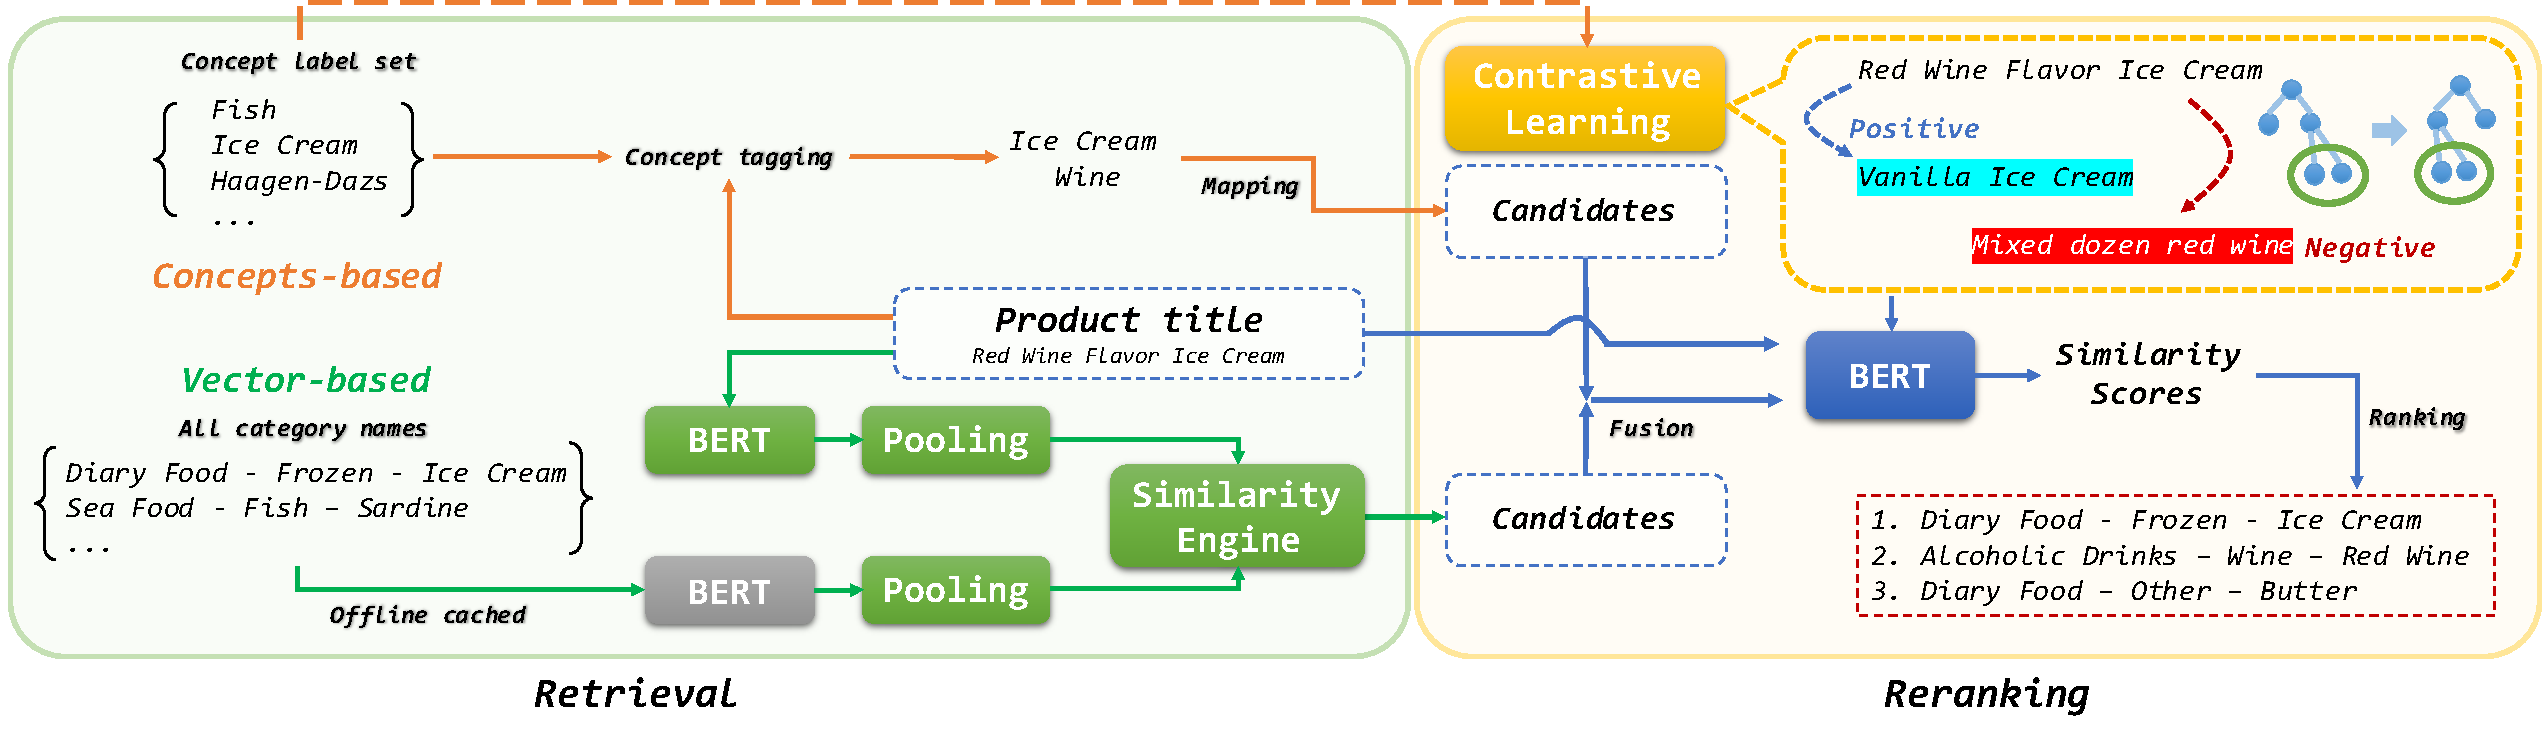
\includegraphics[width=0.99\textwidth]{aaai_fig2}
    \caption{An Overview of our proposed \textit{Taxonomy-agnostic Label Retrieval (TaLR)} framework, containing a \textit{Retrieval} and a \textit{Reranking} stage. Our \textit{Retrieval} stage is based on vector similarity and complements with concept information heuristically. In the next \textit{Reranking} stage, generated candidates are ranked by a scoring engine with contrastive information.}
    \label{fig:pipeline}
\end{figure*}

% \subsection{Task Reformulation}
A single product categorization task on taxonomy $G_i$ ($i=1$) is a traditional classification task, in which the training data and test data are organized in tuples 
$$
\mathcal{S}=\{(X_i^{(1)}, y_i^{(1)}), (X_i^{(2)}, y_i^{(2)}),...,(X_i^{(m_i)}, y_i^{(m_i)}),...\}.
$$
Each $X_i$ in $\mathcal{S}$ represents the title of one product and $y_i$ is the corresponding class node in the categorical taxonomy tree.

In \textit{DMPC} problem, when $i \geq 2$, to unify the training data and the inference procedure cross $G_i$, 
% we aim to match $X_i$ and $y_i$. 
we reformulate classification as the matching between $X_i$ and $y_i$. 
While traditional classifiers regard $y_i$ as meaningless label ordinals, we instead treat them along the path of top-bottom taxonomy nodes equivalently with the product title as free text. 
In this reformulated text semantic similarity matching task, the data samples are:
$$
\mathcal{S}_i=\{(X_i^{(1)}, y_i^{(1)}, Y_{\mathbbm{1}}^{(1)}),...,(X_i^{(m_i)}, y_i^{(m_i)}, Y_{\mathbbm{1}}^{(m_i)}),...\},
$$
$$
\mathcal{S}=\{\mathcal{S}_1, \mathcal{S}_2,...,\mathcal{S}_i\},
$$
where $Y_{\mathbbm{1}}\in \{0, 1\}$ is an indicator denoting whether the text pair $X_i$ and $y_i$ is matched ($Y_{\mathbbm{1}}=1$) or not ($Y_{\mathbbm{1}}=0$).

% This reformulation is especially advantageous to simultaneously (i) capture the semantic relatedness of product titles and label texts and (ii) handle multiple taxonomies \& taxonomy evolving issues in a zero-shot manner without re-training once a unified system is well established.
% ,considering that the label text already contains rich information of this category.